\chapter{Ontology Similarity}


We notice that simple keyword of skill name matching is far from enough, because job description and resume are both written in human language, even the same concepts, they could be written in different ways. For example, Table~\ref{tab:resume_jd}  is part of the resume of a job seeker, and part of a job description:

\begin{table}[ht]
\caption{Resume and Job Description} % title of Table
\centering % used for centering table
\begin{tabular}{ | p{8cm} | p{7cm} | }
 \hline
   \textbf{Part of Resume}                 &   \textbf{Part of Job Description}   \\ \hline

    B.S. degree in computer science \newline
    5+ years Java \newline
    2+ year   C++  \newline
    Some experience in Oracle database \newline
    Other experience like: \newline
    Hibernate, JBOSS, JUnit, Tomcat etc.
  &
  BS degree above   \newline
  4+ years Java  \newline
  Some experience of Python   \newline
    Mysql, MS-SQL   \newline
    Java web application Server   \newline
    OOA/OOD   \\
 \hline
\end{tabular}
\label{tab:resume_jd} % is used to refer this table in the text
\end{table}

If just looking at the text, we can find the resume has few common words with the job description.  But from the view of an experienced engineer, the candidate is pretty matching the job. Because relational databases Oracle and Mysql are very similar, OOA/OOD is the same meaning of many years of Java and C++ experience, and Tomcat and JBOSS are two Java web applications servers.  If we use key word matching, the system won't give a good matching result in this very common situation. So when design the new ontology matching algorithm, we have such considerations:

\begin{enumerate}
    \item How to normalize the same concept with different name or spelling
    \item If one concept in the job description but there is no the same one in the resume, how to calculate the similarity between its related concepts.
    \item If one concept in the job description has multiple similar concepts in the resume, how to summarize total similarity of them.
    \item When calculating the similarity between resume and job description, how to give weights to each concepts.
\end{enumerate}

\section{Ontology Construction}

Semantic web have been a hot research topic in these years, thousands of domain ontologies had created~\cite{ding2004swoogle}. A paradigmatic example is WordNet~\cite{fellbaum1998wordnet}, is a general purpose thesaurus, that contains more than 100,00 general English concepts. But currently, there is no IT technology ontology build for recruiting purpose.  ACM has created a poly-hierarchical ontology that can be utilized in semantic web applications~\cite{acm2012class}.

\begin{figure}[htbp]
  \centering
  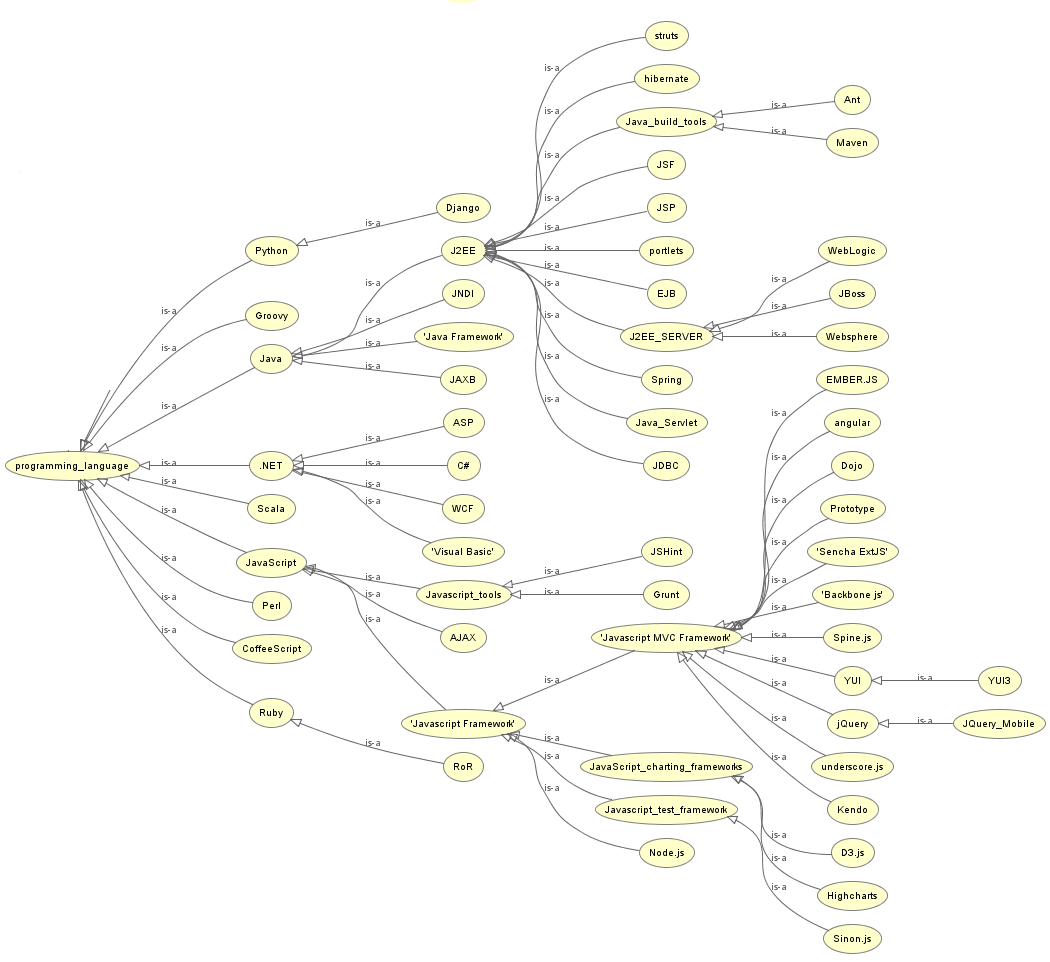
\includegraphics[scale=0.7]{images/ontology_pro.png}
  \caption{Part of Ontology}
  \label{fig:ontology_pro}
\end{figure}

\section{Ontology-based semantic similarity}

The Ontology technics had also been used in some JRSs, which provide a formal specification of a shared conceptualization~\cite{guarino1998formal}.

There are three kinds Ontology-based similarity measure had been studied, they are:

\begin{enumerate}
    \item Edge counting approaches.
    \item Feature-based measures.
    \item Measures based on Information Content.
\end{enumerate}

\subsection{Edge counting approaches}
We could view ontology as a directed graph, in which the nodes are the concepts, the edges are taxonomic relation, like (is-a). Rada, et al.,~\cite{rada1989development} measure the similarity by the distance of two nodes in the graph. So the semantic distance of two concepts a and b will be:
$$ dis_{rad}(a,b) = min |path_i(a,b)| $$

Wu and Palmer ~\cite{wu1994verbs} realized that the depth in the taxonomy will impact the similarity measure of two nodes, because the more deeper of the nodes are in the tree, the semantic distance is smaller. So they gave a new measure of ontology:
$$ sim_{w\&p}(a,b) = \frac{2 \times N_3}{N_1 + N_2 + 2 \times N_3} $$
$N_1$ and $N_2$ is the numbers of is-a links from each term to their Least Common Subsumer(LCS), $N_3$ is the number of is-a links of the LCS to the root of the ontology.

Based on the same idea, Leacock and Chodorow~ \cite{leacock1998combining} also proposed similarity measure that combined distance Np between terms a and b and the depth $D$ of the taxonomy.
$$ sim_{l\&c}(a,b) = -\log (Np/ 2D) $$

\subsection{Feature-based measures}

\subsection{Feature-based measures}


\subsection{Ontology-based semantic similarity in JRSs}
Proactive~\cite{lee2007fighting} used two kinds of ontology, job category and the company information. The system used ontology checker to classify the job information, stored the domain knowledge and calculated the weight value in recommendations.

Kumaran et al~\cite{kumaran2013towards} also used ontology to calculate the similarity between job criteria and candidates's resume in their system~\cite{kumaran2013towards}. The similarity equation they used are:
$$ M\left ( i_1, i_2 \right ) = \frac{\sum_{k=1}^{n} Sim\left (p_{k}^{i1},  p_{k}^{i2} \right ) * W_{k}^{i2}}{\sum_{k=1}^{n} W_{k}^{i2}}  $$
The similarity function $Sim(p_1, p_2)$ is defined as follows:
$$ Sim(p1, p2) = \begin{Bmatrix}
1, & if~similarity~of~p1~and~p2 \geqslant t\\
0, & otherwise
\end{Bmatrix} $$

Fazel \cite{fazel2009semantic} used a hybrid approach to matching job seekers and job postings, which takes advantage of the benefits of both logic-based and ontology-based matching. In his paper the description logics (DL) is used to represent the candidate and job opening, and the ontology is used to organize the skills in a skill taxonomy. He gave an equation to calculate the matching degree:
$$ sim\left(P ,j \right) = \sum x_{ij} \times u(ds_i) $$

where, $x_{ji}$ is the Boolean variable indicating whether desire i is satisfied by applicant $A_{j}$ in the set of all qualified applications.

Liu and Dew~\cite{liu2004using} used RDF to represent and store the expertise of experts , and a RDF-based Expertise Matcher could retrieves the experts whose expertise include the required concept.


\section{statistical-based Ontology Similarity Measure }
In this thesis, I proposed a new statistical-based ontology similarity measure. In most of job descriptions, they will list many skills the positions required. From observation, we could find that related skills always exist in a job description simultaneously, e.g. HTML and CSS are always required together. Furthermore, the distance between two concepts is also a good measure of the relevance of them. We could see this phenomenon in table~\ref{tab:skillinsent}, which include some skills requirement sentences from some job desertions :

\begin{table}[ht]
\caption{Some sentences Job Description} % title of Table
\centering % used for centering table
\begin{tabular}{ | p{15cm}  | }
 \hline
    1. A high-level language such as Java, Groovy, Ruby or Python; we use Java and Groovy extensively \newline
    2. HTML5/CSS3/JavaScript, web standards, jQuery or frameworks like AngularJS would be great \newline
    3. HTML CSS and Javascript a must  \newline
    4. Experience with AJAX, XML, XSL, XSLT, CSS, JavaScript, JQuery, HTML and Web Services   \\
 \hline
\end{tabular}
\label{tab:skillinsent} % is used to refer this table in the text
\end{table}

We could see from the table, the technical close related concepts are always bing together.
Based on such observation, we give a new statistical-based Ontology Similarity Measure. Two concepts $a$ and $b$ in the ontology,   their similarity $S_{a,b}$ could be the ratio of two factors:

\begin{enumerate}
    \item The ratio of the number of documents they exist together $N_{a \cap b}$ to the number of documents have a least one them $N_{a \cup b}$.
    \item The average $\log$ value of their minimum distance $mindis(doc,a,b)$ in documents that have them both.
\end{enumerate}

$$ S(a,b) = \frac{  N_{a \cap b} / N_{a \cup b} }{avg(\log_2( mindis(doc,a,b) + 1 ))} $$

We only apply this measure on the concepts pair if:
\begin{enumerate}
    \item The two concepts have the same direct
    \item One concepts is the super  of another.
\end{enumerate}
We set the restriction because the position of the concept in the ontology is defined based on their technical similarity to others. Similar techniques will assigned into a same category, they should share the same technology base, and one could be a alternate to the other. For example, we put EJB and Hibernate in the same category, because they are both J2EE persistence layer technologies, and both have the O/R mapping concept. If the applicant is familiar one of them, they could master the other very quickly. Another example, like Grail and Django, they are both web frameworks, and share some web design philosophies, but one is  designed for Java web application and the other is created for Python web application. So if one developer has some some experience with one of them, he/she still need spend a lot of time to learn the other to overcome the gap between programming languages. We could see the two examples of in figure:




If distance between two concepts are further than above situation we generally believe they are not related skills. The algorithm to calculate the similarity of two concepts is in algorithm ~\ref{alg:alg_similarity}.

\begin{algorithm}
\caption{Get Stat Similarity}
\label{alg:alg_similarity}
\KwIn{$Docs$�� $term1$, $term2$}
\KwOut{$similarity$}
$total=0$;
$hastwo=0$;
$dislist=\left [ ~~ \right ]$\;
\For{$i=1;~i~\le~len(Docs);~i++$}
{
  \If{ $ Docs_i~has~at~least~one~term $ }
    {
     $ total~+=~1 $ \;
     \If{ $ Docs_i~has~both~terms $ }
        {
           $ hastwo~+=~1 $ ;
           $ mindis~=~ minimium\_distance~(Docs_i, term1, term2) $ \;
           $ dislist.~add  ~\left(  log_2( mindis + 1 ) \right) $ \;
        }
    }
}
$ factor1~=~hastwo~ /~ total $  \;
$ factor2~=~ avg(dislist) $  \;
return $factor1 ~/~ factor2$\;
$ ~~ $
\end{algorithm}

To evaluate this measure, we select 99999 job descriptions, and 99 terms to see the result. We got the relevance matrix in table~\ref{tab:dismatrix} by using the algorithm. Considering the skill HTML, the most relevance skills in order are CSS, Javascript, and jQuery,  which is correct from the perspective of a experienced developer. The other example is Java, the most relevant skill in the matrix is JSP, which is the same as the technical relevance.

\begin{table}

\caption{Skills Similarity Table}
\begin{tabular}{ c | c c c c c c c c }
 \hline
  Term       & Javascript & jQuery &  HTML  &  CSS   &  Java  & Python &  Ruby  &  JSP    \\  \hline
  Javascript &     1      & 0.1981 & 0.2087 & 0.2439 & 0.0665 & 0.0189 & 0.023  & 0.0253   \\
    jQuery   &   0.1981   &   1    & 0.0979 & 0.1328 & 0.0439 & 0.0142 & 0.0266 & 0.0232    \\
     HTML    &   0.2087   & 0.0979 &   1    & 0.3569 & 0.0473 & 0.0175 & 0.023  & 0.0103   \\
     CSS     &   0.2439   & 0.1328 & 0.3569 &   1    & 0.0537 & 0.0153 & 0.0181 & 0.015    \\
     Java    &   0.0665   & 0.0439 & 0.0473 & 0.0537 &   1    & 0.0498 & 0.0287 & 0.075    \\
    Python   &   0.0189   & 0.0142 & 0.0175 & 0.0153 & 0.0498 &   1    & 0.1333 & 0.0025   \\
     Ruby    &   0.023    & 0.0266 & 0.023  & 0.0181 & 0.0287 & 0.1333 &   1    & 0.012    \\
     JSP     &   0.0253   & 0.0232 & 0.0103 & 0.015  & 0.075  & 0.0025 & 0.012  &   1      \\
 \hline
\end{tabular}
\label{tab:dismatrix}
\end{table}



